\section{Introduction}
\label{sec:intro}

Linear interpolation in sRGB display space models the additive mixing of lights, not the subtractive mixing of pigments. For paint-like media, three differences are routinely visible. First, blue and yellow pigments produce green, whereas blue and yellow lights produce a desaturated neutral. Second, complementary pigments produce muted browns, olives, and dark violets, whereas complementary lights tend toward gray. Third, dark pigments lightened with white remain chromatic and shift in hue, whereas an RGB interpolation desaturates toward gray. None of these behaviors follows from a linear combination of display values; \cref{fig:overview} illustrates them for a deep blue pigment mixed with a bright yellow pigment and with white.

The physical reference for pigment mixing is the Kubelka--Munk (K--M) two-flux model. For an opaque layer, the reflectance is $\Rinf(\kappa)=1+\kappa-\sqrt{\kappa^{2}+2\kappa}$ with $\kappa=K/S$, and Duncan showed that the absorption and scattering coefficients of a mixture superpose linearly in concentration \cite{kubelka1931,duncan1940}. Combined with an illuminant and the CIE standard observer, the model reproduces the qualitative and much of the quantitative behavior of pigmented layers \cite{haase1992,wyszecki2000}. Its use in interactive software is nevertheless limited by the interface rather than by the forward model: K--M requires per-pigment spectra, which are not available for an arbitrary RGB color, and mixing two RGB inputs requires inverting the model numerically. In our measurement, the RGB-to-pigment inversion dominates the cost of a spectral mixing operation by a factor of about $10^{5}$ relative to the analytic model introduced here (\cref{sec:runtime}). A further constraint is gamut: some RGB colors cannot be produced by any mixture of available pigments \cite{pointer1980}.

Mixbox \cite{sochorova2021} made K--M-based mixing practical by learning a seven-dimensional latent representation of each RGB color from measured pigment spectra, mixing the latents linearly, and decoding back to RGB with precomputed $256^{3}$ tables. The resulting model reproduces pigment behavior closely and is used as the reference in this work. Its mapping is trained and table-based, and the reference implementation is distributed under a non-commercial license; these properties motivate an analytic alternative, not a replacement for the measured data on which the reference is built.

This paper describes Pigment-Based Mixing (PBM), an analytic model that operates directly on sRGB display values. PBM retains the structural elements of K--M/Duncan mixing---concentration-weighted absorption and scattering, a cross-channel mixing matrix, and a mutual-absorption correction---and adds a repair layer that compensates for the one structural limitation of K--M mixing in display-value space: the scattering term of a near-white color dominates the mixture denominator and washes out the absorption of a dark pigment (\cref{sec:defect}). The repair layer consists of three continuously blended mechanisms: a per-channel power-law target for dark-plus-light mixtures, an additive harmonic correction for complementary pairs, and a soft role assignment that makes the full model exchange-symmetric.

We state the scope of the model explicitly. PBM is \emph{reference-calibrated}: its constants are obtained by inverting and fitting the output of Mixbox~2.0, whose latent space was trained on measured pigment spectra. The model is therefore an approximation of the reference, and its relation to real paint is bounded by the reference's own relation to real paint. We use the term \emph{physics-inspired} only to describe the structural correspondence to K--M/Duncan mixing; none of the fitted constants is derived from pigment physics, and the evaluation does not include measurements of physical paint samples.

\paragraph{Design objectives.}
We evaluate the model against three objectives that we take to be relevant for interactive software:
\begin{enumerate}[label=R\arabic*.,leftmargin=2.2em]
\item operate on sRGB display values, with RGB input and RGB output and without spectral data or additional per-pixel channels;
\item accept all RGB colors, return the inputs exactly at $\alpha=0$ and $\alpha=1$, and vary continuously with the inputs;
\item be fully analytic: no lookup tables, no trained data, and no iteration, so that the model can be reimplemented independently.
\end{enumerate}

\paragraph{Contributions.}
\begin{itemize}
\item An analytic two-stage model for pigment mixing in sRGB display-value space that combines a K--M/Duncan-structured core with a continuously blended repair layer (\cref{sec:model}).
\item A trigonometric-free harmonic correction: a linear model over seventeen channel-ratio features, so that the whole model uses only arithmetic, powers, and square roots (\cref{sec:repair}).
\item A reproducible parameter-estimation procedure, with the harmonic coefficients obtained in closed form by least squares and the remaining scalars by coordinate descent (\cref{sec:estimation}).
\item An ablation and gate-sensitivity study, plus measurements of endpoint identity, neighborhood continuity, exchange symmetry, and runtime (\cref{sec:evaluation}).
\item An evaluation against Mixbox~2.0 with an explicit in-sample/held-out split and bootstrap confidence intervals, and a cross-validation against an independent synthetic spectral world (\cref{sec:results,sec:synthetic}).
\item An explicit account of what the evaluation does not establish (\cref{sec:threats,sec:limitations}).
\end{itemize}

\Cref{tab:positioning} summarizes the positioning. The remainder of the paper reviews the background (\cref{sec:background}), formalizes the model (\cref{sec:model}), describes parameter estimation (\cref{sec:estimation}), reports the evaluation (\cref{sec:evaluation}), and discusses limitations (\cref{sec:limitations}).

\begin{table}[t]
\centering
\small
\caption{Positioning with respect to the design objectives R1--R3 and measured accuracy against Mixbox~2.0 (mean $\Delta E_{00}$; in-sample T5 and held-out T3, \cref{sec:results}).}
\label{tab:positioning}
\begin{tabular}{lccccc}
\toprule
Model & R1 & R2 & R3 & T5 mean & Held-out T3 mean \\
\midrule
PBM (this work) & \checkmark & \checkmark & \checkmark & 2.26 & 2.72--2.85 \\
Mixbox 2.0 \cite{sochorova2021} & \checkmark & \checkmark & $\times$ (trained $256^{3}$ LUT) & reference & reference \\
RGB interpolation & \checkmark & \checkmark & \checkmark & 8.13 & 3.27--3.46 \\
Raw K--M superposition & \checkmark & \checkmark & \checkmark & 10.30 & 3.92--4.01 \\
\bottomrule
\end{tabular}
\end{table}

\begin{figure}[t]
\centering
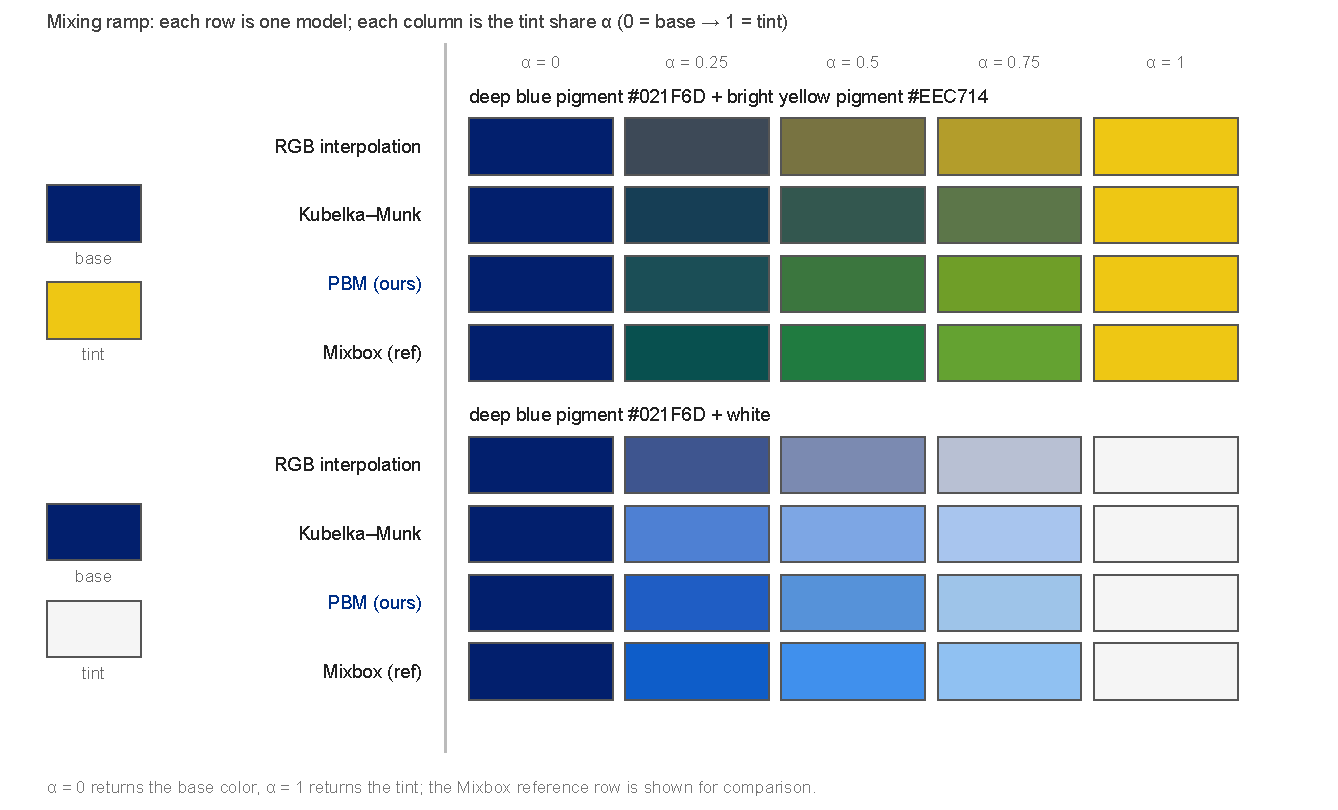
\includegraphics[width=\linewidth]{fig1-mixing.pdf}
\caption{Mixing behavior of RGB interpolation, spectral K--M, PBM, and the Mixbox reference. Top: a deep blue pigment mixed with a bright yellow pigment. Bottom: the same deep blue mixed with white. Each row is one model; each column is the tint share $\alpha$ ($\alpha=0$ returns the base color, $\alpha=1$ the tint). The K--M row is the synthetic spectral truth of \cref{sec:synthetic}: synthetic pigment spectra mixed by two-constant Duncan superposition, with the rendered colors of the pure pigments as inputs. PBM follows the same qualitative families (yellow $\times$ blue $\rightarrow$ green; deep $+$ white remains chromatic).}
\label{fig:overview}
\end{figure}
